\documentclass[a4paper]{article}


%page setting
\usepackage[left=25mm, right=25mm, top=25mm, bottom=25mm]{geometry}

%pakages
%\usepackage[colorlinks=true]{hyperref}
\usepackage{hyperref}
\usepackage{url}
\usepackage{graphicx}
\usepackage{float}
\usepackage{amsfonts}
\usepackage{amsmath}
\usepackage{amssymb}

\usepackage{enumerate}
\usepackage{fancyhdr} %footer-header
%------underline setting--------
\usepackage{ulem}

%--------Table-related commands------
\usepackage{array} %To automatically break longer lines of text within cells, define fixed-width columns
\usepackage[table,xcdraw]{xcolor}

%\usepackage{multirow}
\usepackage{tabularx} % length of table
\usepackage{caption} %space btw caption and table

\usepackage{booktabs}
% produce heavier lines as table frame (\toprule, \bottomrule) and lighter lines within a table (\midrule).

%link: https://texblog.org/2017/02/06/proper-tables-with-latex/
\newcolumntype{V}{>{\bf\centering\arraybackslash} m{0.2\linewidth} } %Repeat column type
%------------------
\usepackage{stackengine}

%--------------Tikz-------------------------------
\usepackage{import}
\usepackage{tikz}
\usepackage{tikz-3dplot}
\usepackage{subfigure}

\usetikzlibrary{shapes.geometric} %draw the flow chart

\usetikzlibrary{positioning} % https://tex.stackexchange.com/questions/94386/package-pgf-math-error-unknown-operator-o-or-of

\usetikzlibrary{automata} %for graph-automata

\usepackage{pgfplots} %for plotting data
%-----------------------------------------------
% PACKAGES for \tkzDefPoints,\tkzPolygon
%-----------------------------------------------
\usepackage{tkz-euclide}
\usepackage{siunitx} %to display angle in degree \ang{180}
\usepackage{fourier} %\widehat{A}
\usetkzobj{all}

\usepackage{verbatim} % a  drawing of a tetrahedron inscibed in a parallelepipe from https://www.overleaf.com/project/5dc97a9a3af030000156a35f
%-------------------------
%\usepackage[nottoc, notlot, notlof]{tocbibind}

%\usepackage{cite}
%\usepackage{natbib} % 
%\usepackage[numbers,sort&compress]{natbib} % sort of citation
\usepackage{pdfpages}

\usepackage{biblatex}
\addbibresource{citation.bib}



%-------------- page editors -----------------------
%\renewcommand{\baselinestretch}{1.5}
\pagestyle{fancy}
\fancyhead{}
%\fancyfoot{}
\renewcommand{\headrulewidth}{0pt}
\renewcommand{\footrulewidth}{1pt}
%------underline setting--------
\renewcommand{\ULdepth}{1.8pt}
%%==============================
%%
%%==============================
% for only 1st example
\makeatletter
\newenvironment{tikzlegend}[1][]{%
   \begingroup
     \csname pgfplots@init@cleared@structures\endcsname
     \pgfplotsset{#1}}{\csname pgfplots@createlegend\endcsname
   \endgroup
}
\def\addlegendimage{\csname pgfplots@addlegendimage\endcsname}
\makeatother
%-------------------------


\begin{document}

%-------------------------
\tableofcontents
\thispagestyle{empty}
\clearpage

\setcounter{page}{1}

%%==============================
%%			CONTENT
%%==============================

% 1st example
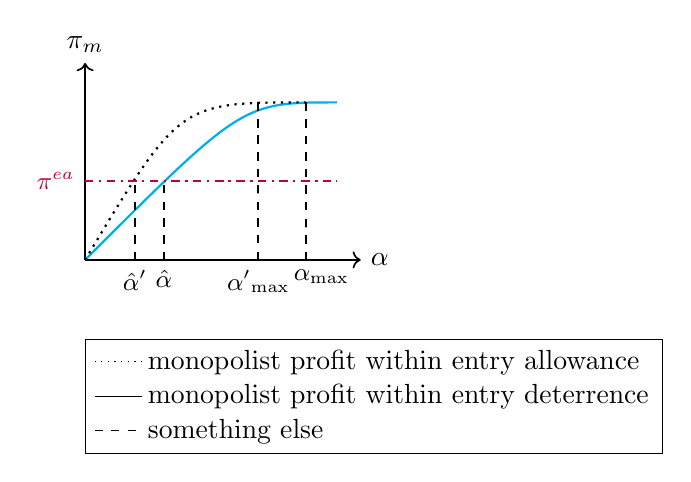
\begin{tikzpicture}
   \draw[semithick,->] (0,0) -- (3.5,0) node[right] {$ \alpha $};
   \draw[semithick,->] (0,0) -- (0,2.5) node[above]  {$ \pi_m $};  
 
   \path[thick,cyan,draw]     (0,0) node[right]{} .. controls (2,2) .. (3.2,2);
   \path[thick,dotted,draw]   (0,0) node[right]{} .. controls (1.2,2) .. (2.8,2);
   \path[thick,dashed,draw]   (2.2,0) node[below]{\small $\alpha{'}_{\max}$} .. controls (2.2,0) .. (2.2,2);
   \path[thick,dashed,draw]   (0.631,0) node[below]{\small $\hat{ \alpha}{'}$} .. controls (0.631,1) .. (0.631,1);
 
   \path[thick,dashdotted,draw,purple]   (0,1) node[left]{\small $\pi^{ea}$}
     .. controls (2,1) ..     (3.2,1);
   \path[thick,dashed,draw]   (2.8,2) node[above]{}
     .. controls (2.8,0) ..   (2.8,0);
   \path[thick,dashed,draw]   (3,0) node[below]{\small $\alpha_{\max}$}
         .. controls (3,0) .. (3,0);
   \path[thick,dashed,draw]   (1,0) node[below]{\small $\hat{\alpha}$}
         .. controls (1,1) .. (1,1);
 
   \begin{tikzlegend}[legend entries={monopolist profit within entry allowance,
      monopolist profit within entry deterrence,something else},
        legend style={at={(0,-1)},anchor=north west}, legend cell align=left]
     \addlegendimage{dotted,sharp plot}
     \addlegendimage{sharp plot}
     \addlegendimage{dashed, sharp plot}
   \end{tikzlegend}
\end{tikzpicture}

\clearpage
\newpage
\section{Flowchart}
\begin{center}
	\input{Flowchart}
\end{center}

%----------------------------------
\section{Nodes}
\begin{center}
	\tikzset{
	level/.style={sibling distance=35mm/#1},
	treenode/.style={align=center,inner sep=0pt},
	% Black nodes
	node_black/.style={treenode,circle,black,draw=black,very thick,text width=0.5cm},
	% Red nodes
	node_red/.style={treenode,circle,red,draw=red,very thick,text width=0.5cm},
	% Blue nodes
	node_blue/.style={treenode,circle,blue,draw=blue,very thick,text width=0.5cm},
	% Nil nodes
	node_nil/.style={treenode,rectangle,fill=black,minimum width=0.3cm,minimum height=0.3cm}
}
\begin{tikzpicture}

\node[node_red] (z){$S$}
  child {node[node_black] (a) {$R$}								%%% Right
    child[black] {node[node_black]  (b) {$R$}
      child {node (b1) {$\vdots$}
       child {node[node_black] (b11) {$R$}}
      }
      child {node (b2) {$\vdots$}
       child {node[node_black] (b12) {$U$}}
      }
    }
    child[black] {node[node_black] (g) {$D$}
      child {node (g1) {$\vdots$}
       child {node[node_black] (g11) {$R$}}
      }
      child {node (g2) {$\vdots$}
       child {node[node_black] (g12) {$U$}}
      }
    }
  }
   child[red] {node[node_red] (d) {$L$}                    %%%% LEft - the shortest parth
      child[black] {node[node_black]  (e) {$L$}
        child {node (e1) {$\vdots$}
         child {node[node_black] (e11) {$R$}}
        }
        child {node (e2) {$\vdots$}
         child {node[node_black] (e12) {$L$}}
        }
      }
      child[red] {node[node_red] (f) {$D$}
        child[black] {node (f1) {$\vdots$}
         child[black] {node[node_black] (f11) {$U$}}
        }
        child[red] {node (f2) {$\vdots$}
         child[red] {node[node_red] (f12) {$G$}}
        }
      }
    }
    child[black] {node[node_black] (m) {$U$}      %%% Up
      child {node[node_black]  (n) {$U$}
        child {node (n1) {$\vdots$}
         child {node[node_black] (n11) {$R$}}
        }
        child {node (n2) {$\vdots$}
         child {node[node_black] (n12) {$L$}}
        }
      }
      child {node[node_black] (o) {$L$}
        child {node (o1) {$\vdots$}
         child {node[node_black] (o11) {$U$}}
        }
        child {node (o2) {$\vdots$}
         child[blue] {node[node_blue] (o12) {$R$}}
        }
      }
    }
  child[black] {node[node_black]  (j) {$D$}   %%% Down
    child {node[node_black] (k) {$D$}
      child {node {$\vdots$}
       child[blue] {node[node_blue] (k11) {$R$}}
      }
      child {node {$\vdots$}
       child {node[node_black] (k12) {$D$}}
      }
    }
    child {node[node_black] (l) {$L$}
    child {node {$\vdots$}
     child {node[node_black] (l11) {$U$}}
    }
    child {node (c){$\vdots$}
     child {node[node_black] (l12) {$L$}
            child [grow=right] {node (r) {$level^n$} edge from parent[draw=none]
              child [grow=up] {node (s) {$\vdots$} edge from parent[draw=none]
                child [grow=up] {node (t) {$level^2$} edge from parent[draw=none]
                  child [grow=up] {node (u) {$level^1$} edge from parent[draw=none]
                   child [grow=up] {node (u) {$root$} edge from parent[draw=none]}
                                   }
                                 }
                               }
                               }
            }
          }
         }
};
\path (b) -- (g) node [midway] {$\cdots$};\path (n) -- (o) node [midway] {$\cdots$};
\path (e) -- (f) node [midway] {$\cdots$};
\path (k) -- (l) node [midway] {$\cdots$};
\path (b11) -- (b12) node [midway] {$\cdots$};
\path (g11) -- (g12) node [midway] {$\cdots$};\path (n11) -- (n12) node [midway] {$\cdots$};
\path (e11) -- (e12) node [midway] {$\cdots$};\path (o11) -- (o12) node [midway] {$\cdots$};
\path (f11) -- (f12) node [midway] {$\cdots$};
\path (k11) -- (k12) node [midway] {$\cdots$};
\path (l11) -- (l12) node [midway] {$\cdots$};

%\begin{tikzlegend}[legend entries={monopolist profit within entry allowance,
%      monopolist profit within entry deterrence,something else},
%        legend style={at={(0,-1)},anchor=north west}, legend cell align=left]
%     \addlegendimage{dotted,sharp plot}
%     \addlegendimage{sharp plot}
%     \addlegendimage{dashed, sharp plot}
%\end{tikzlegend}   
   
\end{tikzpicture}

%% take notes

\vskip 0.5cm

\begin{tikzpicture}
\draw (-0.5,-2.5) rectangle(6,0.7);
\draw[-][draw=black, very thick] (0,0) -- (1.5,0);
\draw (1.8,0) node[node_black]{S}  ;
\draw (3.7,0) node{Possible path} ;
\draw[-][draw=blue, very thick] (0,-1) -- (1.5,-1);
\draw (1.8,-1) node[node_blue]{R} ;
\draw (4.3,-1) node{Achieving same path} ;
\draw[-][draw=red, very thick] (0,-2) -- (1.5,-2);
\draw (1.8,-2) node[node_red]{G} ;
\draw (3.5,-2) node{Final path} ;
\end{tikzpicture}
%\vskip 0.5cm
\end{center}

%----------------------------------
\newpage
\section{Grap-Automata}
\begin{figure}[h!]
	\begin{center}
		%--- using \usetikzlibrary{automata}
%\newpage
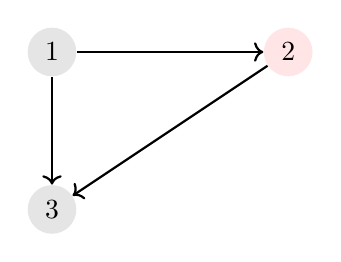
\begin{tikzpicture}
	\tikzstyle{vertex}=[circle,fill=black!10]
	\tikzstyle{selected vertex}=[vertex,fill=red!10]
	\tikzstyle{edge}=[->,thick]
	
	\node[vertex](v1) at (0,0){1};
	\node[selected vertex](v2) at (3,0){2};
	\node[vertex](v3) at (0,-2){3};	
	
	\draw[edge](v1)--(v2);
	\draw[edge](v1)--(v3);
	\draw[edge](v2)--(v3);	
\end{tikzpicture}
\caption{Example1}

\vspace{30pt}

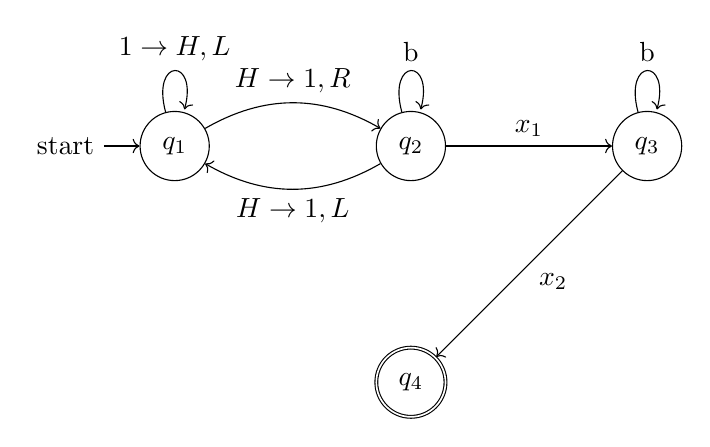
\begin{tikzpicture}[->,node distance=3cm,auto]
	\node[initial,state](A){$q_1$};
	\node[state](B)[right of=A]{$q_2$};
	\node[state](C)[right of=B]{$q_3$};
	\node[state,accepting](D)[below of=B]{$q_4$};
	
	\path(A)edge[loop above]node{$1\rightarrow H,L$}(A)
			edge [bend left] node{$H \rightarrow 1,R$}(B)
		 (B)edge[loop above]node{b}(B)
		    edge [bend left] node{$H \rightarrow 1,L$}(A)
			edge node{$x_1$}(C)
    	 (C)edge[loop above]node{b}(C)
    	    edge node{$x_2$}(D)
	;	
\end{tikzpicture}
\caption{Example2}

\vspace{30pt}

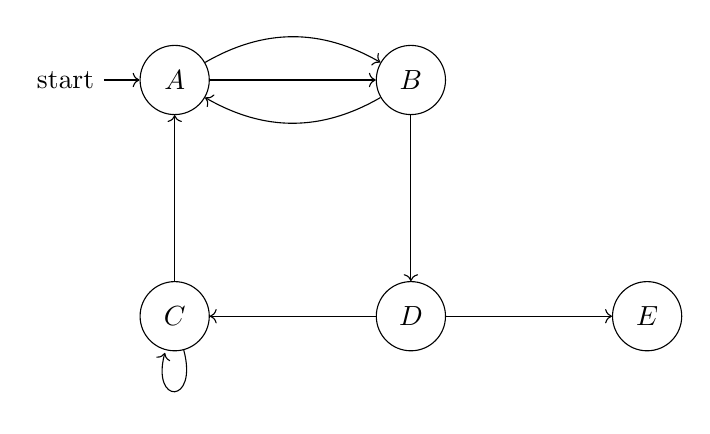
\begin{tikzpicture}[->,node distance=3cm,auto]
	\node[initial,state](A){$A$};
	\node[state](B)[right of=A]{$B$};
	\node[state](C)[below of=A]{$C$};
	\node[state](D)[below of=B]{$D$};
	\node[state](E)[right of=D]{$E$};
	
	\path(A)edge[bend left](B)
	        edge(B)		 
		 (B)edge[bend left](A)
			edge(D)
    	 (C)edge(A)
    	    edge[loop below](C)
    	 (D)edge(C)
    	    edge(E)  
	;	
\end{tikzpicture}
\caption{This is node graph}
	\end{center}
\end{figure}

%----------------------------------
\newpage
\section{Plotting Data}
\begin{figure}[ht]
	\begin{center}
		%\newpage
\begin{tikzpicture}
    \begin{axis}[name=plot, xlabel={x(Ns/m)},ylabel={y(J)},ymin=0,ymax=1.6]
    
    \addplot[black,mark=triangle*] table{./data/friction.txt};\label{f}
    \addplot[red,mark=o] table{./data/generator.txt};\label{g}
    \addplot[blue] table{./data/simulated_total.txt};\label{s}
    \addplot[green,dashed] table{./data/theoretical_total.txt};\label{t}
	
	% Define two points for drawing an arrow to the "matched" point
%    \node[] (C) at (axis cs: 1,0.5) {};
%    \node[] (B) at (axis cs: 2.5,0.5) {};
    \end{axis}
	
	% Create a node to act as the legend  
    \node[anchor=north,fill=white,draw=black] (legend) at 
    ($(plot.north east)-(0 mm, 1 mm)$){
    	\begin{tabular}{l l}
        	f & \ref{f} \\
	        g & \ref{g} \\
    	    s & \ref{s} \\
        	t & \ref{t} \\
	    \end{tabular} 
	    };
    
%	\draw[triangle 45-] (C.east)--(B.west);
%	\node[anchor=west] (label) at (B) {matched};

\end{tikzpicture}
\caption{Example of plotting data1}

\vspace{30pt}

\begin{tikzpicture}
    \begin{axis}[name=plot, xlabel={x(Ns/m)},ylabel={y(J)},ymin=0,ymax=1.6]
    
    \addplot[black,mark=triangle*] table{./data/friction.txt};\label{f}
    \addplot[red,mark=o] table{./data/generator.txt};\label{g}
    \addplot[blue] table{./data/simulated_total.txt};\label{s}
    \addplot[green,dashed] table{./data/theoretical_total.txt};\label{t}
	
	% Define two points for drawing an arrow to the "matched" point
    \node[] (C) at (axis cs: 1,.5) {};
    \node[] (B) at (axis cs: 2.5,.5) {};
    \end{axis}
	
	% Create a node to act as the legend  
    \node[anchor=north,fill=white,draw=black] (legend) at ($(plot.north)-(0 mm, 1 mm)$) {\begin{tabular}{l l l l}
        f & \ref{f}  & g & \ref{g} \\
        s & \ref{s}  & t & \ref{t} \\
    \end{tabular} };
    
	\draw[triangle 45-] (C.east)--(B.west);
	\node[anchor=west] (label) at (B) {matched};

\end{tikzpicture}
\caption{Example of plotting data2}

\vspace{30pt}
	\end{center}
\end{figure}

%----------------------------------
\newpage
\section{Rotation Geometry}
\begin{figure}[ht]
	\begin{center}
		%---
%
%
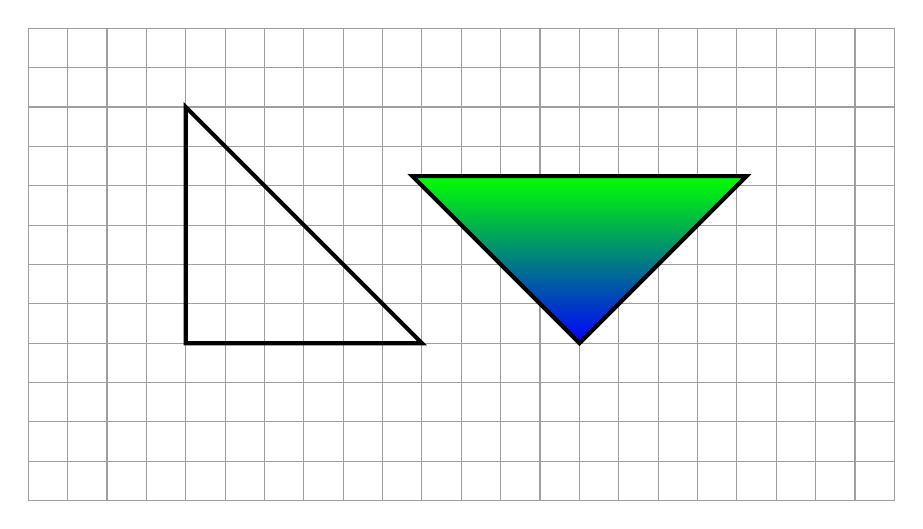
\begin{tikzpicture}
	\draw[step=0.5,gray!75](-2,-2) grid(9,4); %from (-2,-2) to (9,4)
	\draw[line width=1.5pt](0,0)--(3,0)--(0,3)--cycle;
	\draw[line width=1.5pt, xshift=5cm, rotate=45, bottom color = blue, top color=green](0,0)--(3,0)--(0,3)--cycle;
\end{tikzpicture}
\caption{Rotation Triangular}


	\end{center}
\end{figure} 

%--------- draw SimplePolygon.tex-------
\section{Draw Simple Polygon}
\begin{figure}[ht]
	\begin{center}
		
\begin{tikzpicture}[scale=1.5, transform shape]
	
			\tkzInit[xmin=-3,xmax=4.5, ymin=-.5, ymax=2.8]
			\tkzClip
			
			\tkzDefPoint(0,0){A}
			\tkzDefPoint(4,0){B}
			\tkzDefPoint(130:3){C}
			
			
			
			\tkzDefLine[orthogonal=through C](A,B)\tkzGetPoint{c}
			\tkzInterLL(A,B)(C,c)\tkzGetPoint{C'}
			
	
			\tkzMarkAngle[size=.5,arrows=->,>=stealth,color=red](B,A,C)
			\tkzMarkAngle[size=.4,arrows=->,>=stealth,color=blue](C,A,C')
			\tkzMarkRightAngle[size=.3,fill=blue!20,draw opacity=0](A,C',C)
			
			
			\tkzDrawSegment[dashed](C,C')
			\tkzDrawLine[add=0cm and 1cm,dashed](A,C')
			
			
			
			\tkzDrawPolygon(A,B,C)
			\tkzDrawPoints(A,B,C,C')
			\tkzLabelPoints[below](A,C')
			\tkzLabelPoints[right](B)
			\tkzLabelPoints[above](C)
			
			\begin{scope}[font=\footnotesize]
			\tkzLabelSegment[below](A,B){$c$}
			\tkzLabelSegment(A,C){$b$}
			\tkzLabelSegment[above](B,C){$a$}
			\tkzLabelSegment[left](C,C'){$h$}
			\tkzLabelAngle[pos=.7](B,A,C){$\widehat{A}$}
			\tkzLabelAngle[pos=1.1,below](C,A,C'){$\ang{180}-\widehat{A}$}
			\end{scope}
			
\end{tikzpicture}
\caption{Draw Polygon with  }
	\end{center}
\end{figure} 

%--Parallelepiped.tex--
\section{Draw Rectangle Polygon}
\begin{figure}[ht]
	\begin{center}
		\input{Parallelepiped}
	\end{center}
\end{figure
\newpage
\section{Draw Sphere}
\input{Stereographic}



\printbibliography
\end{document}